\begin{figure}[H]
  \centering
  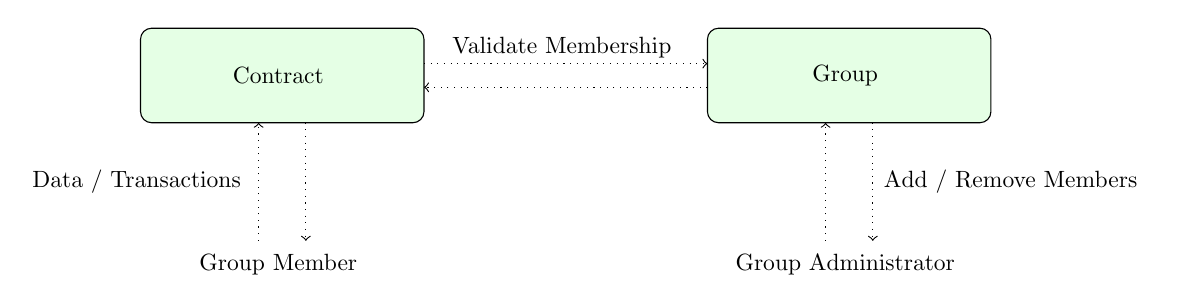
\begin{tikzpicture}[scale = 0.6, every node/.style={scale = 0.85}, every node/.append style={fill = white, rounded corners = 2pt, inner sep = 2pt, align = center}]

  \draw [rounded corners, fill=green!10] (-3, 1) rectangle (3, -1);
  \node [fill=green!10] at (0, 0) { Contract };

  \node at (-3, -2.25) { Data / Transactions };
  \draw [ -> , dotted] (-0.5, -3.5) -- (-0.5, -1);
  \draw [ -> , dotted] (0.5,  -1) -- (0.5,  -3.5);

  \node at (0, -4) { Group Member };

  \draw [rounded corners, fill=green!10] (9, 1) rectangle (15, -1);
  \node [fill=green!10] at (12, 0) { Group };

  \node at (15.5, -2.25) { Add / Remove Members };
  \draw [ -> , dotted] (11.5, -3.5) -- (11.5,    -1);
  \draw [ -> , dotted] (12.5,   -1) -- (12.5,  -3.5);

  \node at (12, -4) { Group Administrator };

  \node at (6, 0.6) { Validate Membership };
  \draw [ -> , dotted] (3,  0.25) -- (9,  0.25);
  \draw [ -> , dotted] (9, -0.25) -- (3, -0.25);

  \end{tikzpicture} \\
  \caption{
  	How a group interacts with an identity's data
  }
  \label{fig:archi_group_interactions}
\end{figure}
